\section{Comparing a plain GAN and a Wasserstein GAN}

\subsection{Networks architecture}
	The discriminator and the generator in both the GAN and the WGAN are implemented using convolutional neural networks. The architecture is visualized in Figure~\ref{fig:gan_arc}. As we can see, the generator networks are identical while the architecture of the discriminators has some minor differences. For examples, the size of the convolutional filter is smaller in the WGAN discriminator. Also, the WGAN discriminator's output is not a probability of an image being real anymore but rather a $2 \times 2 \times 1 $ tensor which is solely used to compute the loss functions of the WGAN networks. As already discussed in Section~\ref{sec:batch_norm}, almost all layers of the networks have a batch normalization. Implementation of these models can be found on Github~\url{https://github.com/melkonyan/BA_WassersteinGAN}. 
\begin{figure}[h]
	\includegraphics[width=\textwidth]{figures/architecture}
	\caption{Architectures of the GAN and the WGAN used in this paper.}
	\label{fig:gan_arc}
\end{figure}
\subsection{Proposed evaluation method}
Unfortunately, the generative adversarial metric discussed in Section~\ref{sec:gam} can not be applied to compare a plain GAN with a WGAN. This is due to the fact that the output of a WGAN discriminator can not be interpreted as a probability that a sample is real. Therefore, we can not compute the $\epsilon(D_{WGAN}(x_{real}))$ and $\epsilon(D_{WGAN}(G_{GAN}(z)))$ terms of Equations~\ref{eq:gam_real} and \ref{eq:gam_gen} respectively. I have tried to use an approach inspired by the GAM but instead of computing the error rates $\epsilon(\cdot)$ on a test dataset I have plotted discriminators' losses during the training process. Here is the summarized procedure: 
\begin{enumerate}
	\item Do several training steps of both the GAN and the WGAN.
	\item Log the WGAN discriminator's performance 
		\begin{enumerate}
			\item Compute the WGAN discriminator's loss using images generated by the GAN generator.
			\item Compute the WGAN discriminator's loss using its own generator
		\end{enumerate}	
	\item Log the GAN discriminator's performance
		\begin{enumerate}
			\item Compute the GAN discriminator's loss using images generated by the WGAN generator.
			\item Compute the GAN discriminator's loss using its own generator
		\end{enumerate}
	\item Go to Step 1.
\end{enumerate}
Before taking a look at the results let us discuss possible outcomes of the procedure described above, which are visualized in Figures~\ref{fig:cd_wgan_wins},~\ref{fig:cd_equal},~\ref{fig:cd_gen_overfit},~\ref{fig:cd_dis_overfit}. 
In the normal case one of the two following scenarios will happen:
\begin{enumerate}
	\item The desired scenario, in which one of the generators produces images that are harder to distinguish for both discriminators. In this case we can assume that the generator can produce images of a better quality. An example of the corresponding loss curves is shown in Figure~\ref{fig:cd_wgan_wins}.	
	\item If both generators perform equally well, all the loss curves will be approximately identical, as shown in Figure~\ref{fig:cd_equal}.
\end{enumerate}

	\begin{figure}[h!] 
		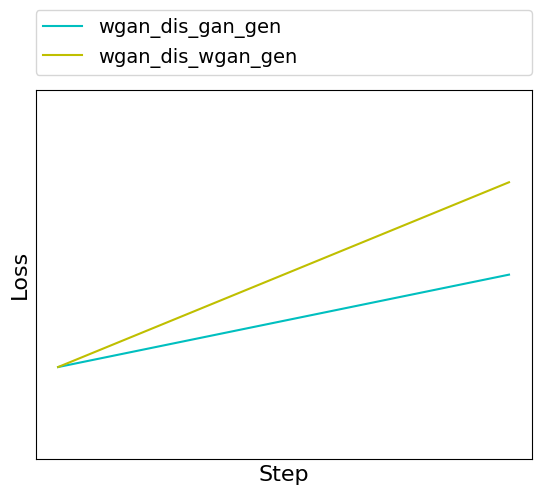
\includegraphics[width=0.5\textwidth]{figures/ex/wgan_wins_wgan_dis}
		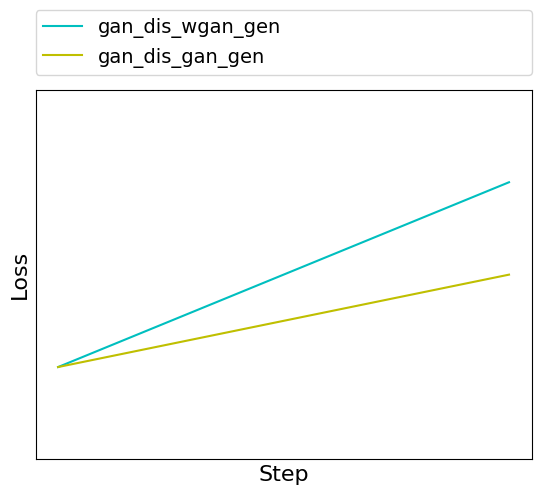
\includegraphics[width=0.5\textwidth]{figures/ex/wgan_wins_gan_dis}
		\caption{Both WGAN and GAN discriminators losses are bigger when competing against WGAN generator. A sign that the WGAN generator produces better images.}
		\label{fig:cd_wgan_wins}
	\end{figure}
	\begin{figure}[h!]
		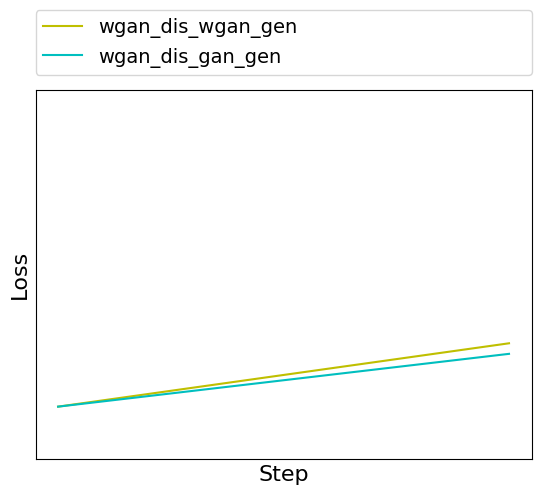
\includegraphics[width=0.5\textwidth]{figures/ex/equal_wgan_dis}
		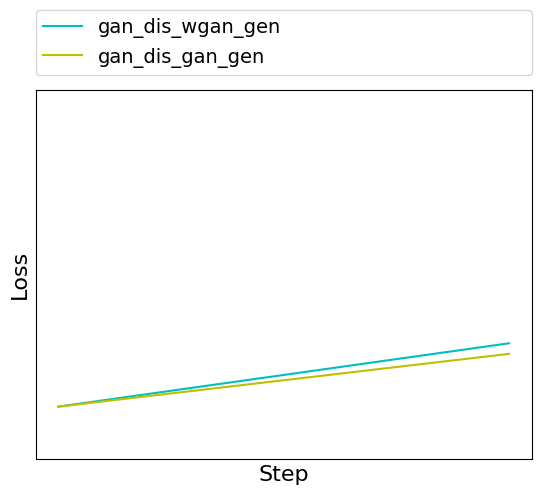
\includegraphics[width=0.5\textwidth]{figures/ex/equal_gan_dis}
		\caption{Both WGAN and GAN discriminators perform almost equally well on the both generators.}
		\label{fig:cd_equal}
	\end{figure}
	
	
However, it can also happen, that either a discriminator or a generator overfits in one or even both GANs. There are lots of possible combinations, here are some examples:
\begin{enumerate}
	\item Both generators overfit with respect to their own discriminators. This means, that they will be able to produce images that do not look better from a human perspective, but are tuned to fool the respective discriminator. In this case we will see graphs like in Figure~\ref{fig:cd_gen_overfit}.
	\item It is also possible that the discriminators overfit in a sense that instead of analyzing the structure of real images they remember peculiarities present in the images produced by their generators. In this scenario plots will resemble those shown in Figure~\ref{fig:cd_dis_overfit}.
	\item The trickiest case is when the WGAN discriminator overfits and at the same time the GAN generator, or vice versa. Unfortunately, as shown in Figure~\ref{fig:cd_gen_dis_overfit}, in this case the loss plots could look very similar to the case where WGAN generator just performs better.
\end{enumerate}

	\begin{figure}[h!] 
		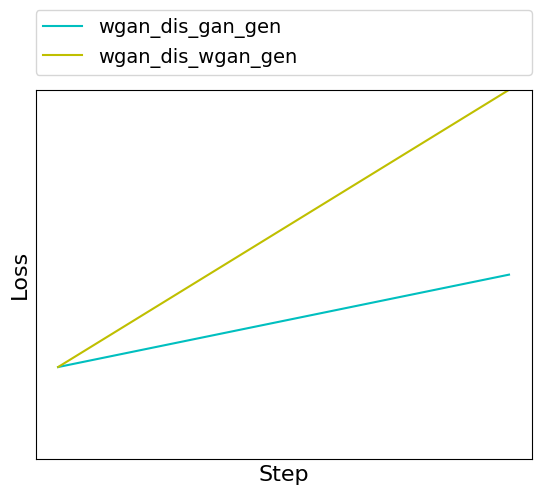
\includegraphics[width=0.5\textwidth]{figures/ex/gen_overfit_wgan_dis}
		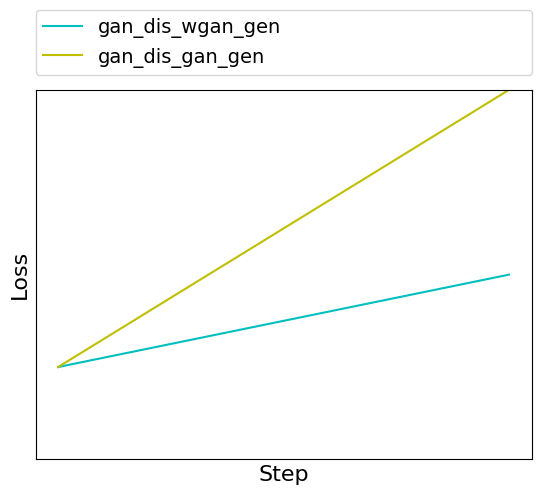
\includegraphics[width=0.5\textwidth]{figures/ex/gen_overfit_gan_dis}
		\caption{Both WGAN and GAN discriminators losses are bigger when competing against own generator. A sign that generators overfit against own discriminators.}
		\label{fig:cd_gen_overfit}
	\end{figure}
	\begin{figure}[h!] 
		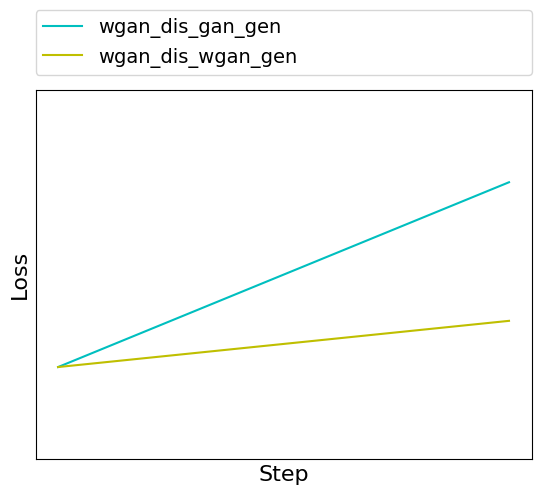
\includegraphics[width=0.5\textwidth]{figures/ex/dis_overfit_wgan_dis}
		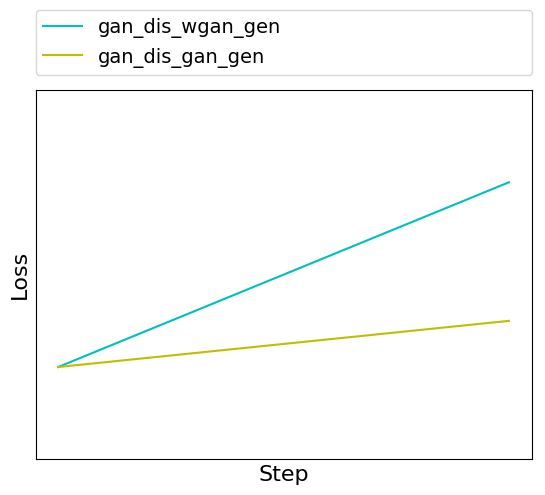
\includegraphics[width=0.5\textwidth]{figures/ex/dis_overfit_gan_dis}
		\caption{Both WGAN and GAN discriminators losses are bigger when competing against each other's generator. A sign that discriminators overfit against own generators.}
		\label{fig:cd_dis_overfit}	
	\end{figure}	
	\begin{figure}[h!] 
		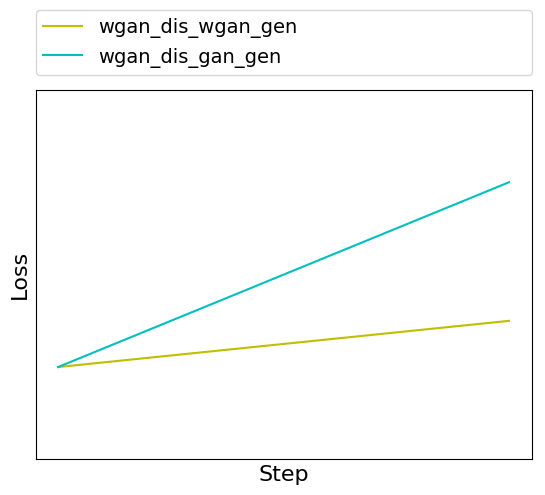
\includegraphics[width=0.5\textwidth]{figures/ex/gen_dis_overfit_wgan_dis}
		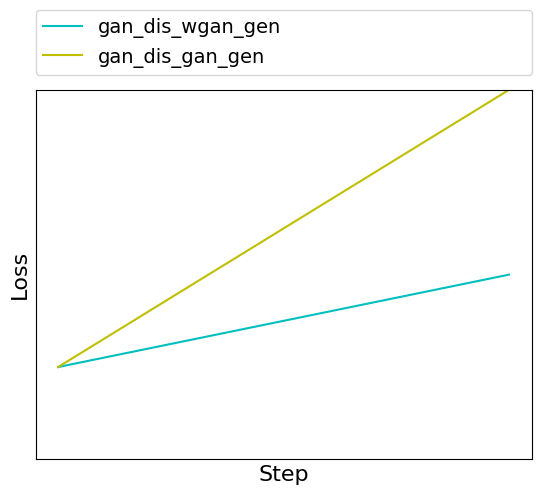
\includegraphics[width=0.5\textwidth]{figures/ex/gen_dis_overfit_gan_dis}
		\caption{Both the WGAN and GAN discriminators losses are bigger when competing against GAN generators. However, in this case the GAN discriminator and the WGAN generator overfit.}
		\label{fig:cd_gen_dis_overfit}
	\end{figure}
As we have seen, even in the case where one generator causes more problems for both discriminators, this can be a consequence of overfitting. So, normally, we would have to do additional tests to verify whether this is the case or not. Such a verification can be done by applying the same technique to two instances of the same network type, e.g. two WGANs. If after the additional verification we conclude that there is no overfitting, then we can finally claim that one generator performs relatively better. Moreover, in practice it turns out that multiple runs can produce different results even when using the same hyper-parameters. This happens because overfitting can be a result of a poor weight initialization. Therefore, each test has to be repeated several times and produce congruent results. 

There are several key differences when comparing this modified metric to the original generative adversarial metric. First, as already said, the GAM can not be applied to GANs whose discriminators do not output a valid probability distribution, which is the case with the WGAN. On the other hand, the GAM can be applied to a fully trained network, while each run of the modified metric requires both networks to be trained from scratch. However, as I have observed during my experiments, one has to train the networks several times due to occasional overfitting. Also, the modified metric provides information about the loss at different times of the training process. This can provide additional information, because if two networks change the lead multiple times during the training, it means that they can not be really compared.  

\subsection{Results}
The results of applying the modified generative adversarial metric are shown in Figure~\ref{fig:cd_wgan_vs_gan}. As we can see, after a significant amount of training steps the WGAN discriminator is able to distinguish images produced by its own and by the GAN discriminator equally well. On the other hand, the GAN discriminator almost constantly performs much better on its own generator. This may suggest that the GAN discriminator overfits. 
\begin{figure}[h!]
	\begin{subfigure}[b]{0.5\textwidth}
		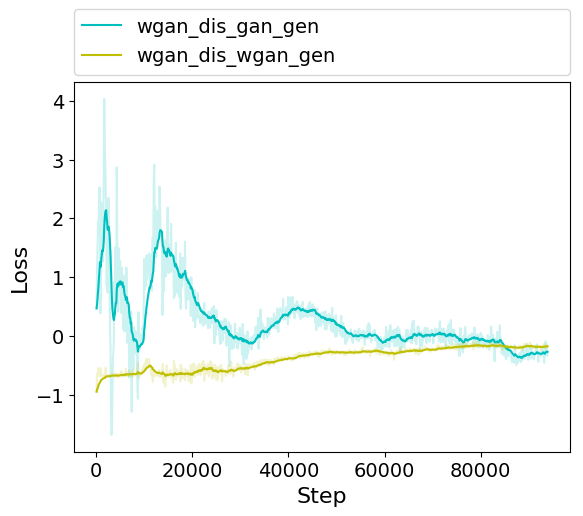
\includegraphics[width=\textwidth]{figures/cross_dis/trial16_wgan_dis_gan_gen}
	\end{subfigure}
	\begin{subfigure}[b]{0.5\textwidth}
		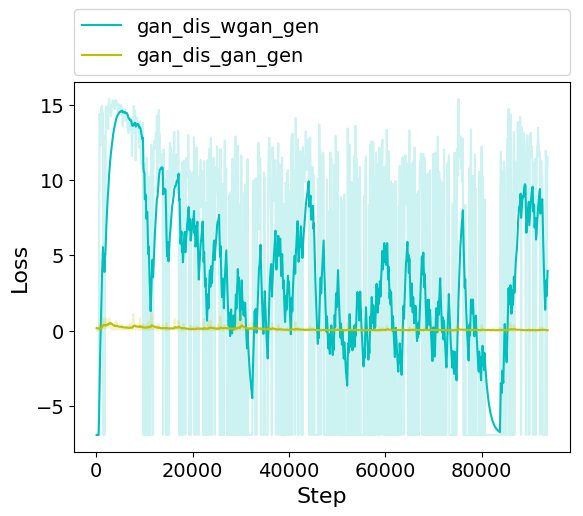
\includegraphics[width=\textwidth]{figures/cross_dis/trial16_gan_dis_wgan_gen}
	\end{subfigure}
	\caption{Results of applying the modified adversarial metric on a GAN and a WGAN. As we can see the GAN discriminator almost constantly performs worse when judging images produced by the WGAN generator, on the other hand the WGAN discriminator performs equally well on both generators.}
	\label{fig:cd_wgan_vs_gan}
\end{figure}

\begin{figure}[h!]
	\begin{subfigure}[b]{0.5\textwidth}
		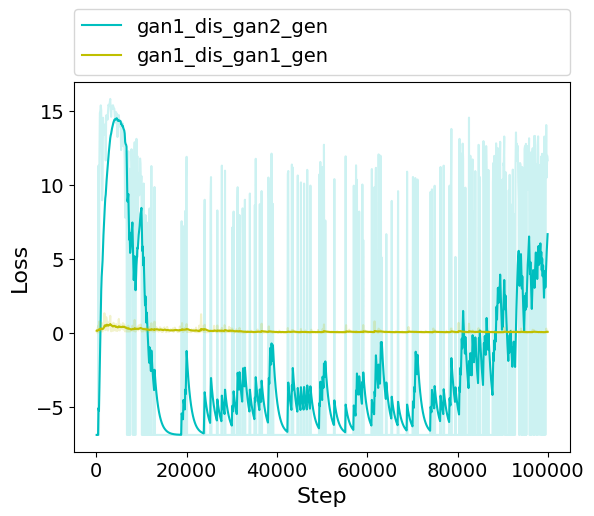
\includegraphics[width=\textwidth]{figures/cross_dis/trial15_gan1_dis_gan2_gen}
	\end{subfigure}
	\begin{subfigure}[b]{0.5\textwidth}
		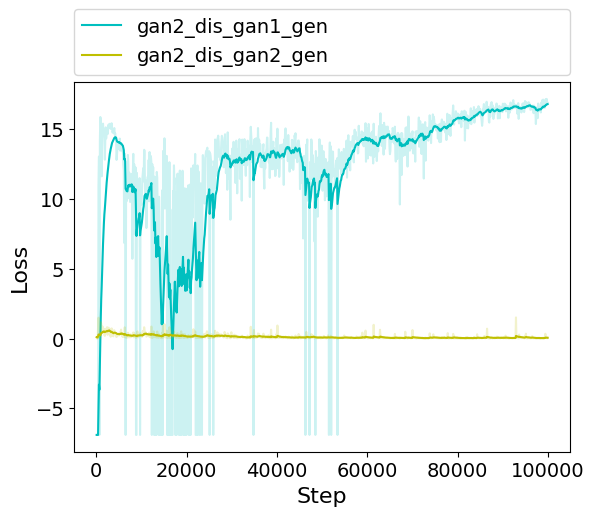
\includegraphics[width=\textwidth]{figures/cross_dis/trial15_gan2_dis_gan1_gen}
	\end{subfigure}
	\caption{Results of applying the modified adversarial metric on two GANs. Both discriminators can better distinguish images from their own generators}.
	\label{fig:cd_gan_vs_gan}
\end{figure}

To further investigate this hypothesis I have used the same metric to compare two GANs. The corresponding results are shown in Figure~\ref{fig:cd_gan_vs_gan}. While loss plots are oscillating, the trend is that after at some point of the training process GAN discriminator performs better on its own generator. On the other hand, when comparing two WGAN discriminators, it turned out that they perform equally well on both generators, as shown in Figure~\ref{fig:cd_wgan_vs_wgan}. All experiments were conducted several times and the corresponding plots can be found in Appendix~\ref{app:results}.
\begin{figure}[h!]
	\begin{subfigure}[b]{0.5\textwidth}
		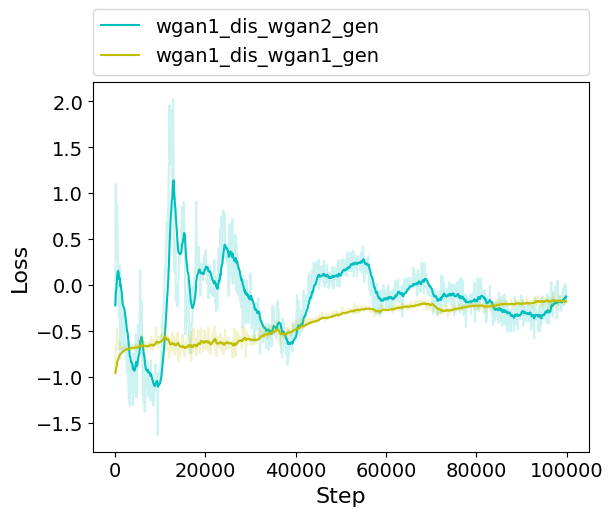
\includegraphics[width=\textwidth]{figures/cross_dis/trial17_wgan1_dis_wgan2_gen}
	\end{subfigure}
	\begin{subfigure}[b]{0.5\textwidth}
		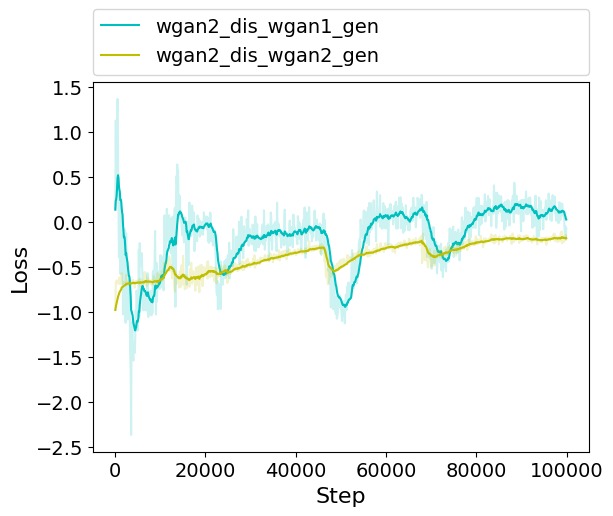
\includegraphics[width=\textwidth]{figures/cross_dis/trial17_wgan2_dis_wgan1_gen}
	\end{subfigure}
	\caption{Results of applying the modified adversarial metric on two WGANs. Both discriminators can better distinguish images from the foreign generator.}
	\label{fig:cd_wgan_vs_wgan}
\end{figure}

There are two main conclusions that can be drawn from the experiment results. Firstly, since the WGAN discriminator does not show any overfitting behavior, we can use its loss values when measuring both GAN and WGAN generators to claim that they both produce images of the same quality. Those who believe in their own ability to distinguish real and generates faces can take look at the samples generated by both generators, included in Appendix~\ref{app:results}. Furthermore, experiments suggest that the GAN discriminator overfits with respect to its own generator. Therefore, I have conducted more experiments to investigate the decision boundary learned by the GAN discriminator.

\begin{figure}[h]
	\centering
	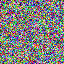
\includegraphics[scale=1]{figures/gan_found_image1}
	
\includegraphics[scale=1]{figures/gan_found_image2}
	
\includegraphics[scale=1]{figures/gan_found_image3}
	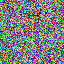
\includegraphics[scale=1]{figures/gan_found_image4}
	\caption{Examples of images that the GAN discriminator considers real.}
	\label{fig:gan_found_images}
\end{figure}

\begin{figure}[h!]
	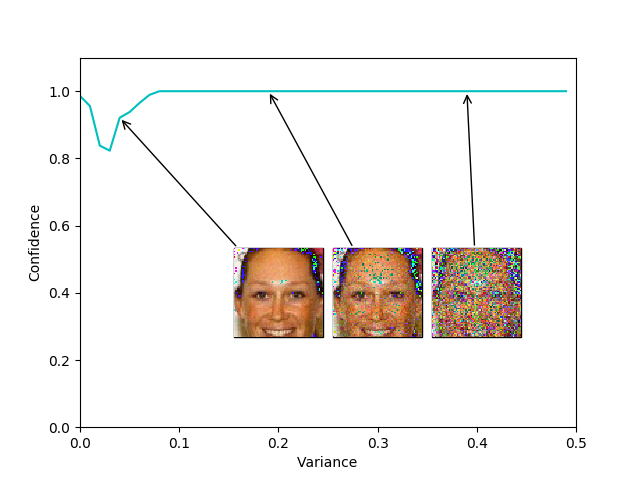
\includegraphics[width=\textwidth]{figures/diversity_gan2_real_dis_real_images}
	\caption{A visualization of how the GAN discriminator's confidence changes when we add a Gaussian noise to a real image sample.}
	\label{fig:changed_real_image_real_dis}
\end{figure}

\begin{figure}[h!]
	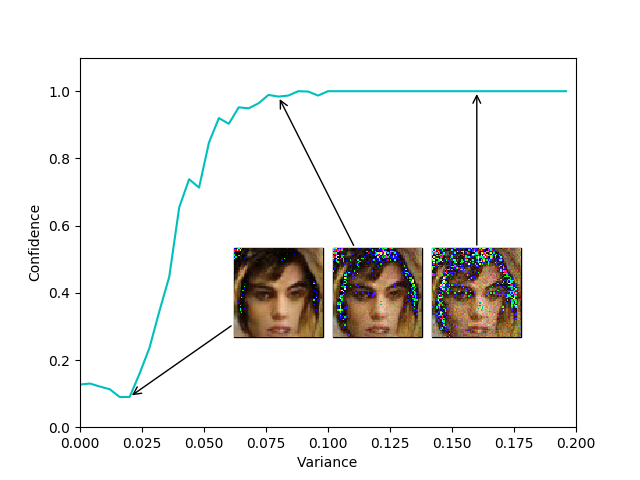
\includegraphics[width=\textwidth]{figures/diversity_gan2_fake_dis_gen_images}
	\caption{A visualization of how the GAN discriminator's confidence changes when we add a Gaussian noise to a generated image sample.}
	\label{fig:changed_gen_image_fake_dis}
\end{figure}

Once a discriminator is fully trained we can search for an image which discriminator will confidently mark as real. We can do it by using gradient descent over the image space, using the output of the discriminator as a loss function:
\begin{equation}
	I^* = \argmax_{I \in R^{64 \times 64 \times 64}} D(I).
\end{equation} 
However, using output directly will result in a very slow learning, because the output of discriminator on a newly initialized random image should be almost zero. Therefore, the sigmoid function used as an activation in the last layer will be saturated and the gradient will vanish. Instead, I used output before activation. Of coarse, the discriminator's output is not a convex function and has numerous local maxima. But by conducting the search multiple times with different initial images we have a chance to find a maxima that will give us a confidence near one. 

However, in practice it turned out that the GAN discriminator's confidence is equal to one almost on the whole image space and it constantly marked randomly generated images as real, like the ones shown in Figure~\ref{fig:gan_found_images}. To further investigate this phenomenon I have tried to add Gaussian noise with different variances to find out how much should I distort an image to decrease the discriminator's confidence:
\begin{align*}
	Z &\sim \mathcal{N}(0, \sigma^2) \\
	\hat{I} &= I + Z.
\end{align*} One would expect that the more noise is added to the image the less likely the discriminator will think the image is real. However, results demonstrated in Figures~\ref{fig:changed_real_image_real_dis} and~\ref{fig:changed_gen_image_fake_dis} suggest the opposite. When an image was distorted to an extent, where the underlying face was hardly visible, the GAN discriminator marked it as real with a confidence equal to one. These results suggest that the loss function of the GAN discriminator has many local minimas in the points corresponding to the generated faces and is equal to one in all the regions that were not observed during the training process. 

These results suggests that we should not use the discriminator network for classifying whether an image is real or not. This is because it does not learn the whole set of possible pictures but rather only those present in the training data set (positive examples) and those produced by its generator (negative examples). So, in the regions not observed during the training process its function can take some arbitrary values, in this case it was equal to one almost everywhere. The most important part of a GAN is the generator network and the discriminator exists only to help the generator to train. 

%\begin{figure}[h]
%	\begin{subfigure}[b]{0.5\textwidth}
%		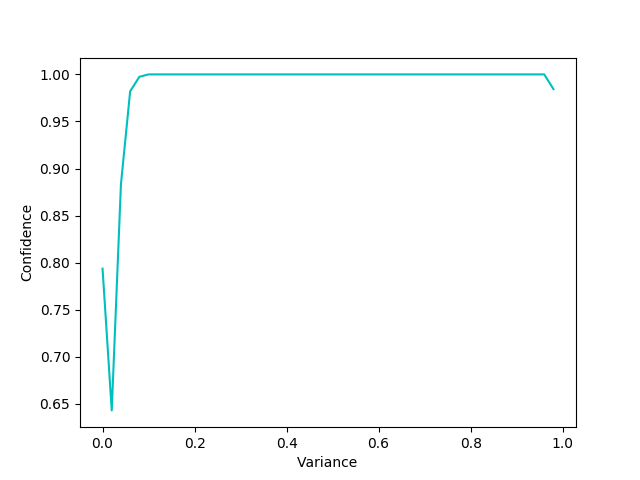
\includegraphics[width=\textwidth]{figures/diversity_gan2_real_dis_gen_images_plot}
%	\end{subfigure}
%	\begin{subfigure}[b]{0.5\textwidth}
%		\centering
%		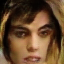
\includegraphics[width=0.45\textwidth]{figures/diversity_gan2_real_dis_gen_imgs_var0}
%		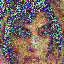
\includegraphics[width=0.45\textwidth]{figures/diversity_gan2_real_dis_gen_imgs_var30}
%		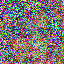
\includegraphics[width=0.45\textwidth]{figures/diversity_gan2_real_dis_gen_imgs_var50}
%		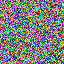
\includegraphics[width=0.45\textwidth]{figures/diversity_gan2_real_dis_gen_imgs_var90}
%	\end{subfigure}
%	\caption{Visualization of how GAN discriminator's confidence changes when we add Gaussian noise to a real image sample.}
%	\label{fig:changed_gen_image_real_dis}
%\end{figure}

%\begin{figure}[h]
%	\begin{subfigure}[b]{0.5\textwidth}
%		\centering
%		
\includegraphics[scale=1]{figures/random_images_fake_1}
%		
\includegraphics[scale=1]{figures/random_images_fake_2}
%		\caption{The images that the GAN discriminator considered fake.}
%	\end{subfigure}
%	\begin{subfigure}[b]{0.5\textwidth}
%		\centering
%		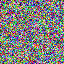
\includegraphics[scale=1]{figures/random_images_real_2}
%		\caption{The images that the GAN discriminator considered real.}
%	\end{subfigure}
%\end{figure}



